% !TEX TS-program = XeLaTeX
% use the following command: 
% $ xelatex -shell-escape -output-driver="xdvipdfmx -z 0" article.tex
% this "-z 0" must be used to suppress compression in XMP Metadata packet 
% all document files must be coded in UTF-8
\documentclass{textolivre}
% for anonymous submission
%\documentclass[anonymous]{textolivre}
% to create HTML use 
%\documentclass{textolivre-html}
% remove all auxiliary files
% find . -name 'tl-article-template.*' ! -name '*.tex' ! -name '*.pdf' ! -name '*.bib' -type f -exec rm {} \;
% HTML compile using make4ht
% $ make4ht -c textolivre-html.cfg -u -x article "fn-in,svg"   # or use `mathjax' instead of `svg' to get LaTeX equation that will be handled by MathJax
% $ bibtex article
% clean and prettify HTML 
% $ tidy -o article-tidy.html --output-xhtml --break-before-br --wrap 0 article.html 2> errs.txt
% https://www.html-tidy.org/documentation/

% Metadata
\begin{filecontents*}{article.xmpdata}
    \Title{Competencia léxica y escritura académica: analíticas de aprendizaje en un curso de escritura universitaria}
    \Author{Gabriel Valdés-León}
    \Language{es}
    \Keywords{Competencia léxica \sep Escritura académica \sep Analíticas de aprendizaje \sep Iramuteq \sep Análisis lexicométrico}
    \Journaltitle{Texto Livre}
    \Journalnumber{1983-3652}
    \Volume{14}
    \Issue{1}
    \Firstpage{1}
    \Lastpage{16}
    \Doi{10.35699/1983-3652.2021.24560}

    \setRGBcolorprofile{sRGB_IEC61966-2-1_black_scaled.icc}
            {sRGB_IEC61966-2-1_black_scaled}
            {sRGB IEC61966 v2.1 with black scaling}
            {http://www.color.org}
\end{filecontents*}

% PDF/A
% - install package icc-profiles
% - it is necessary to convert all image files to PDF/A
%   use ghostscript as shown below:
%   PDF images:
%   $ gs -dPDFA -dBATCH -dNOPAUSE -sColorConversionStrategy=UseDeviceIndependentColor -dCompatibilityLevel=1.4 -sDEVICE=pdfwrite -sProcessColorModel=DeviceCMYK -dPDFACompatibilityPolicy=2 -sOutputFile=figure-a.pdf figure.pdf
%   Other images:
%   $ convert figure.png figure.eps
%   $ gs -dPDFA -dBATCH -dNOPAUSE -sColorConversionStrategy=UseDeviceIndependentColor -dCompatibilityLevel=1.4 -sDEVICE=pdfwrite -sProcessColorModel=DeviceCMYK -dPDFACompatibilityPolicy=2 -dEPSCrop -sOutputFile=figure.pdf figure.eps

\journalname{Texto Livre: Linguagem e Tecnologia}
\thevolume{14}
\thenumber{1}
\theyear{2020}
\receiveddate{\DTMdisplaydate{2020}{08}{09}{-1}} % YYYY MM DD
\accepteddate{\DTMdisplaydate{2020}{10}{05}{-1}}
\publisheddate{\today}
% Corresponding author
\corrauthor{Gabriel Valdés-León}
% DOI
\articledoi{10.35699/1983-3652.2021.24560}
% Abbreviated author list for the running footer
\runningauthor{Valdés-León, G.}

\title{Competencia léxica y escritura académica: analíticas de aprendizaje en un curso de escritura universitaria}
\othertitle{Competência léxica e escrita acadêmica: análise da aprendizagem em um curso de escrita universitário}
\othertitle{Lexical competence and academic writing: learning analytics in a university writing course}

\author[1]{Gabriel Valdés-León \orcid{0000-0001-8807-8838} \thanks{Email: \url{gvaldesl@ucsh.cl}}}
\affil[1]{Universidad de Las Palmas de Gran Canaria, España.}

%\usepackage[backend=biber,style=abnt, ittitles]{biblatex}
%\DeclareLanguageMapping{brazil}{brazil-apa}
\addbibresource{article.bib}     
% use biber instead of bibtex
% $ biber tl-article-template
% $ pdflatex tl-article-template.tex

% set language of the article
\setdefaultlanguage{spanish}
\setotherlanguage{portuguese}
\setotherlanguage{english}

\begin{document}
\maketitle

\begin{poliabstract}
\begin{abstract}
Gracias a la generación de analíticas de aprendizaje, se recogió
información relacionada con el desempeño léxico y escritural en 36 textos
producidos por estudiantes pertenecientes a un curso de escritura de educación
superior. Esta información no solo permitió tomar decisiones pedagógicas en el
corto plazo, sino también planificar una investigación que indagara en la
relación que existe entre ambas competencias. El artículo que aquí se presenta
se hace cargo del segundo desafío planteado, y tiene como objetivo identificar
la relación que existe entre el dominio léxico académico y el nivel de
los textos producidos por este grupo de alumnos a partir de las analíticas de
aprendizaje obtenidas. Para ello, se elaboró un estudio de caso, de tipo
pre experimental y transversal,en el que se compara la calidad de los textos
redactados por los discentes en una tarea de escritura con un estudio
lexicométrico realizado a esos mismo escritos utilizando el software libre
Iramuteq. Los resultados indican que existe una estrecha relación entre léxico
académico y calidad del contenido, pero que el vínculo se vuelve
menos determinante al contrastar léxico académico con la calidad textual de los
trabajos.

\keywords{Competencia léxica \sep Escritura académica \sep Analíticas de aprendizaje \sep Iramuteq \sep Análisis lexicométrico.}
\end{abstract}

\begin{portuguese}
\begin{abstract}
Graças à geração de análises de aprendizagem, informações relacionadas
ao desempenho lexical e escritural foram coletadas em 36 textos produzidos por
alunos deum curso de redação de ensino superior. Essas informações
possibilitaram não apenas tomar decisões pedagógicas em curto prazo, mas também
planejar um estudo que investigasse a relação entre as duas competências. O
artigo aqui apresentado trata do segundo desafio que se coloca, e tem como
objetivo identificar a relação que existe entre o domínio lexical acadêmico e o
nível dos textos produzidos por este grupo de alunos apartir das análises de
aprendizagem obtidas. Para tanto, foi desenvolvido um estudo decaso, do tipo
pré-experimental e transversal, no qual a qualidade dos textos escritos
pelos alunos em uma tarefa de escrita foi comparada com um estudo lexicométrico
realizado sobre essas mesmas escritas no software livre Iramuteq. Os resultados
indicam que existe uma estreita relação entre o léxico acadêmico e a qualidade
do conteúdo, mas quea vinculação se torna menos decisiva ao contrastar o léxico
acadêmico com a qualidade textual dos trabalhos.

\keywords{Competência lexical \sep Escrita acadêmica \sep Análises de aprendizagem \sep Iramuteq \sep Análise lexicométrica.}
\end{abstract}
\end{portuguese}

\begin{english}
\begin{abstract}
Based on learning analytics, information related to lexical and
scriptural performance was collected in 36 texts produced by students belonging
to a higher education writing course. This information not only allowed to make
pedagogical decisions in the short term, but also to plan an investigation on
the relationship between both competences. The article presented here addresses
the second challenge posed, and its objective is to identify the relationship
that exists between the academic lexical domain and the level of the texts
produced by this group of students based on the learning analytics obtained. To
do this, a case study was developed, of a pre-experimental and cross-sectional
type, in which the quality of the texts written by the students in a
writing task is compared with a lexicometric study carried out on those same
writings using thefree software Iramuteq. The results indicate that there is a
close relationship between academic lexicon and content, but that link becomes
less decisive when contrasting academic lexicon with textual quality.

\keywords{Lexical competence \sep Academic writing \sep Learning analytics \sep Iramuteq \sep .Lexicometric analysis.}
\end{abstract}
\end{english}

\end{poliabstract}


\section{Introducción}\label{sec-intro}

La utilización de analíticas de aprendizaje para mejorar los procesos
educativos posee ya un par de décadas, no obstante, la investigación en torno a
su uso se encuentra en pleno auge \cite{caceres2020}. Pese a lo alentador que
esto último pueda parecer, existe aún una considerable distancia entre los
avances de la tecnología y el ámbito educativo, lo que representa un profundo
desaprovechamiento del potencial que tienen las tecnologías de uso diario en el
aprendizaje de los estudiantes, en el mejoramiento de los métodos didácticos y
en la respuesta que espera la sociedad de las instituciones educativas \cite[p. 556]{penalvo2015}. 
Esta distancia se hace aún más patente en espacios formativos
como los que ofrece Sudamérica, por ejemplo,en donde la incorporación de la
tecnología a la educación es aún una tarea pendiente.

Efectivamente, la implementación generalizada de entornos
completamente tecnologizados en las aulas del sur de América, al estilo de los
Entornos Virtuales de Aprendizaje (EVA), parece un sueño aún bastante alejado;
no obstante, sin dejar de lado iniciativas de alta envergadura, como el proyecto
LALA, orientado hacia el uso de analíticas de aprendizaje para mejorar la
educación superior de América Latina, es posible encontrar en la literatura
especializada experiencias que dan cuenta de resultados exitosos que,
generalmente, se encuentran circunscritos a la enseñanza de un tema o de curso
en particular \cite[por ejemplo]{ninoCarrasco2019}.

Actualmente, las analíticas de aprendizaje suelen definirse como un proceso
de medición del comportamiento de los estudiantes en entornos virtuales con el
fin de realizar un seguimiento de su desempeño y, gracias a ello, crear data que
permita tomar decisiones pedagógicas. En palabras de \textcite{Sabulsky2019},
“las analíticas de aprendizaje son dispositivos tecnológicos que se incorporan a
entornos virtuales de interacción, con el fin de registrar las huellas digitales
que dejan quienes participan en ellos, creando grandes bases de datos”.

Si bien la definición anterior sitúa a las analíticas de aprendizaje
inevitablemente
dentro de entornos virtuales, esta investigación adopta una
perspectiva un tanto más amplia, pues las concibe como herramientas que
“procesan datos, analizan estadísticas,generan informes de uso y
proporcionan a profesores y alumnos información sobre
las interacciones del alumno y de su progresión” \cite[p. 185]{conole}. Esto
nos permite considerar que los datos recogidos luego de la experiencia de aula
que forma parte de este estudio, la que se realizó de manera presencial y con
metodologías de aprendizaje'tradicionales' (es decir, sin estar inmersos en un
EVA), pueden enriquecerse con análisis estadísticos proporcionados por
herramientas tecnológicas. Gracias a ello, la información que se ha
obtenido luego del desarrollo de una tarea de escritura por
parte de los 36estudiantes del curso Producción oral y escrita ha sido
analizada desde dos perspectivas:desempeño escritural y desempeño léxico.

Este trabajo se enmarca en los continuos esfuerzos de una universidad
chilena privada por aportar en la formación de los estudiantes de Pedagogía en
castellano a través de la búsqueda permanente de mecanismos de innovación
docente. Como parte de esos esfuerzos, este trabajo tiene como objetivo
identificar la relación que existe entre el dominio léxico académico y el nivel
de los textos producidos por estudiantes de nuevo ingreso a partir de las
analíticas de aprendizaje obtenidas. Para ello, se diseñó un estudio de caso que
contó con la participación de la totalidad de los estudiantes de primer año
de dicha carrera (36 matriculados, año 2019), en el que se analizó información a
través dedos mecanismos: una rúbrica para conocer tanto el nivel de redacción
como el dominio de contenidos; y un análisis lexicométrico llevado a cabo a
través del programa informático Iramuteq, que permitió conocer el manejo del
léxico académico por parte de los estudiantes.


\subsection{La escritura y su relación con el léxico}\label{sec-la-escr}
La escritura es un proceso complejo que va mucho más allá de garabatear
signos sobre un papel. Es una competencia transversal, por tanto, transferible,
que implica un esfuerzo multidimensional (pues contempla los niveles cognitivo,
social e incluso emocional) y que se desarrolla durante toda la vida \cite{Balta2018}.
En este sentido, la escritura – como proceso – involucra una serie de
habilidades que adquieren mayor o menor relevancia dependiendo de la situación
comunicativa en la que se encuentra el hablante y del texto – o producto – que
se quiere elaborar. Así, un texto académico requiere investigar, ordenar,
clasificar, jerarquizar, criticar, adecuar, evaluar..., mientras que textos que
dejan en un segundo plano el valor epistémico de la escritura resultan ser menos
demandantes, al menos en el plano cognitivo \cite{cantis2013,navarro}

La importancia medular que tienen tanto la lectura como la escritura para
el desarrollo humano y, particularmente, para la educación, ha motivado una
considerable cantidad de investigaciones sobre estrategias que permitan
fortalecer estas competencias. Si nos enfocamos en los estudios realizados en
educación superior en el ámbito latinoamericano, es posible identificar “un
aumento progresivo de iniciativas de enseñanza, investigación, publicación,
eventos y esfuerzos de sistematización”\cite{Navarro2016}.

Esta creciente preocupación por los estudios de alfabetización académica
se fundamenta, entre otros aspectos, en el desafío que una nueva cultura
discursiva supone
\begin{quote}
El concepto de alfabetización académica [...] señala el conjunto de nociones
y estrategias necesarias para participar en la cultura discursiva de las
disciplinas así como en las actividades de producción y análisis de textos
requeridas para aprender en la universidad. Apunta, de esta manera, a las
prácticas de lenguaje y pensamiento propias del ámbito académico \cite[p. 410]{cantis2003}.
\end{quote}

Este nuevo escenario plantea también nuevos desafíos en el plano discursivo,
lo que puede desembocar en problemas de rendimiento académico. En
efecto,investigaciones como las de \textcite{Ayala2019,ValdsLen2020} 
señalan que los estudiantes universitarios de primer año suelen evidenciar
debilidades respecto de sus competencias de lectura y escritura al momento de
hacer frente estas nuevas demandas de la educación terciaria. Y uno de los
caminos que surgen desde la didáctica de la escritura puede encontrarse en el
fortalecimiento de las (sub)competencias comunicativas asociadas a la escritura,
entre ellas, la lectura y el léxico.

Los estudios que abordan el léxico como parte de la competencia
comunicativa también han evidenciado un aumento sostenido de publicaciones
académicas que estudian tópicos relacionados con la didáctica, la evaluación y
el aprendizaje del vocabulario \cite{perfetti2001,rufat2016}. No
obstante, al momento de revisar lo que se ha producido en el área, queda en
evidencia que la mayor cantidad de estudios que buscan potenciar la competencia
léxica han surgido bajo el alero de la enseñanza del español como lengua
extranjera (ELE), siendo considerablemente menor el número de trabajos que
apuntan hacia la enseñanza del español como lengua materna.Por su parte,
subdisciplinas lingüísticas como la disponibilidad léxica y la
psicolingüística experimental se han enfocado en temas más acotados como la
medición del léxico disponible y del léxico pasivo, sin relacionar
necesariamente sus resultados con el ámbito educativo \cite{GermanyG2000,echeverria1987,RiffoOcares2014}.

Lo anterior no es más que una evidencia de que la posición protagónica que
ha tomado la competencia léxica como parte de la competencia comunicativa ha
sido reconocida por los docentes de ELE, pero no suficientemente valorada cuando
se trata de didáctica del español como lengua materna, por lo que nos parece que
es un ámbito que resulta necesario fortalecer, sobre todo, considerando los
datos que existen cuando relacionamos competencia léxica, competencias lectoras
y competencias escritura les \cite{GonzaloZapico2016,Zapico2017,kaur,Pinto2019}.

En el plano local chileno, basta con observar los resultados que se han
obtenido tanto en evaluaciones estandarizadas nacionales (e.g., SIMCE) como
internacionales (e.g., PISA) \cite{VillarroelHenrquez2015,FigueroaSeplveda2018}
para comprender la necesidad de reforzar los procesos relacionados
con lectura y escritura a nivel primario, secundario y terciario y,
específicamente, con la formación de los futuros docentes, con énfasis en los
profesores de español como lengua materna.

Hasta este punto, hemos mencionado la importancia que tiene el léxico dentro de
la enseñanza de una lengua, ya sea lengua materna o una segunda lengua, por
ello, resulta imprescindible profundizar en torno a esta competencia.

Existe consenso entre los investigadores especializados en el estudio del
léxico en mencionar a Richards como uno de los primeros lingüistas que abordó
el concepto de competencia léxica, aunque cabe precisar que el autor utilizó la
expresión \textit{knowing a Word} al momento de desarrollar su trabajo \cite{Richards1976,Choudhury2015,Velsquez2016}.
No obstante, más allá de la nomenclatura
utilizada, la propuesta de Richards fue pionera al momento de estudiar cómo las
palabras se relacionan de manera compleja a nivel gramatical, semántico,
sociolingüístico y psicolingüístico \cite{catalan2002}, considerando
también elementos cognitivos, por cierto, dada la perspectiva pedagógica que su
obra posee. De esta manera, \textcite[p. 78--83]{Richards1976} propone ocho premisas que
permitirían guiar procesos de enseñanza de vocabulario:

\begin{enumerate}
\item El vocabulario de un hablante nativo continúa expandiéndose durante su adultez.
\item Conocer una palabra significa conocer el grado de probabilidad de encontrarla y asea de manera oral o escrita.
\item Conocer una palabra implica conocer las limitaciones impuestas a su uso de acuerdo con las variaciones de función y situación.
\item Conocer una palabra significa conocer el comportamiento sintáctico asociado con esa palabra.
\item Conocer una palabra implica conocer su forma subyacente y las derivaciones quede esta palabra pueden surgir.
\item Conocer una  palabra implica conocer la red de  asociaciones entre  esa  palabra  y otras palabras de la lengua.
\item Conocer una palabra significa conocer el valor semántico de esa palabra.
\item Conocer una palabra significa conocer muchos de los otros significados asociados con esa palabra. [la traducción es nuestra]
\end{enumerate}

Como podemos observar, la propuesta de este autor destaca por romper con
una mirada estática frente al estudio del léxico, pues es enfático en señalar
que el aprendizaje del vocabulario no se limita al conocimiento del significado,
forma y derivados de una palabra.

Sin dejar de valorar el aporte de Richards, \textcite[p. 15]{arancibia} menciona
que “[Richards] no distingue entre los diferentes niveles y grados de
conocimiento de la palabra, ni tampoco menciona cómo el aprendiente llega a
adquirir ese conocimiento”. Fue \textcite{natio1990} quien realiza una propuesta en la
que establece una distinción explícita entre el conocimiento receptivo y
productivo del vocabulario, señalando que el nivel productivo involucra niveles
de conocimiento más altos \cite{Choudhury2015}. En esta línea de pensamiento,
\textcite{natio2001} amplía su propuesta y señala que lo que actualmente comprendemos
como competencia léxica implica tres niveles de conocimiento:

\begin{quote}
The terms receptive and productive apply to a variety of kinds of
language knowledge and use. When they are applied to vocabulary, these terms
cover all the aspects of what is involved in knowing a Word. [...]. At the most
general level, knowing a word involves form, meaning and use \cite[p. 40]{natio2001}.
\end{quote}

En las diferentes definiciones que podemos encontrar en la literatura
especializada respecto del concepto de competencia léxica, es posible observar,
con mayor o menor preponderancia, la presencia de estos elementos. Así, por
ejemplo, \textcite[p. 57]{molina2007} define competencia léxica como la
“habilidad para reconocer y usar las palabras de una lengua del mismo modo que
los hablantes nativos lo hacen. Incluye, por tanto, la comprensión de las
diferentes relaciones entre las familias de palabras y las colocaciones comunes
de las palabras”. En esta misma obra, la autora refiere al trabajo de \textcite[p. 152]{catalan2002},
quien señala que la competencia léxica implica, por
una parte, conocer una palabra para poder utilizarla y, por otra, reconocerla y
relacionarla con las demás, tanto en la oralidad como en la escritura. Es
innegable, entonces, que la competencia léxica es multidimensional y compleja y
-- tal como señalaba Richards décadas atrás-involucra un proceso de aprendizaje
progresivo.



\section{Metodología}\label{sec-metodologia}
A continuación, se exponen los principales elementos que conforman
la metodología de este estudio de caso en el que participaron 36 estudiantes
universitarios chilenos.

\subsection{Diseño}\label{sec-diseno}
El diseño de esta investigación se corresponde con un estudio pre experimental
de tipo transversal, ya que que el trabajo se orienta hacia la descripción y el
análisis de variables tal como se presentan en un momento dado, considerando
incluso sus interrelaciones \cite{acuna2006}.

\subsection{Participantes}\label{sec-participantes}
Los criterios de inclusión consideraron, por una parte, la pertenencia al
curso Producción oral y escrita I, en el que estaban inscritos la totalidad de
los estudiantes de primer año cohorte 2019; por otra, la disposición de los
estudiantes por sumarse a este estudio, lo que se tradujo en la aceptación por
escrito mediante un consentimiento informado. En consecuencia, la investigación
contó con la participación de 36 jóvenes universitarios de entre 17 y 26 años.
La actividad curricular en la que se enmarcó el trabajo posee carácter
obligatorio y se caracteriza por tributar a las competencias transversales y
disciplinares del perfil de egreso de la titulación.

\subsection{Actividades pedagógicas}\label{sec-actividades}
Al finalizar el primer semestre del año 2019, la universidad en la que se
realizó esta investigación solicitó a las unidades académicas la implementación
de una evaluación final de carácter integrativo, que permitiera recoger
información relacionada con el nivel de logro alcanzado en el desarrollo de
competencias declaradas en los programas de cada actividad curricular. A raíz de
esto, el desafío para la Escuela de Educación en Castellano fue diseñar
evaluaciones que recogieran información en dos dimensiones:disciplinar, tanto
para lingüística y literatura como para los cursos pedagógicos y deformación
general; transversal, para conocer el nivel de desempeño en competencias clave,
a saber, lectura y escritura.

Los resultados que expone esta investigación han sido obtenidos desde un corpus
de textos producidos por los 36 estudiantes de la cohorte al momento de rendir
la evaluación integrativa del curso Producción oral y escrita I. Esta evaluación
se dividió en dos partes: la primera, que contenía preguntas de alternativas con
selección única,relacionadas con aspectos conceptuales abordados durante el
semestre; la segunda, que invitaba a los estudiantes a elaborar un texto de
opinión a partir de la lectura de un fragmento (páginas 15-22) de Recetas para
escribir, de Daniel Cassany y Antonio García. Esta última sección fue la que se
recopiló para construir el corpus, pues permitió recoger información sobre
producción textual y léxico académico.


\subsection{Variables}\label{sec-variables}
Al momento de examinar los trabajos, se analizó la presencia de léxico
académico,por una parte, y la calidad de los textos, por otra. Para este último
aspecto, se tomaron en cuenta “dominios disciplinares” y “criterios de
producción textual”, aspectos que se detallarán en el \Cref{sec-instru}. Por tanto,
se indagará en la relación entre dominio léxico académico y a) calidad textual
(o, en palabras simples, forma); b) contenido académico (contenido); y c) y
calidad global del texto (forma y contenido).


\subsection{Instrumento}\label{sec-instru}
Los instrumentos utilizados para la recolección y análisis de los datos son
aquellos que se relacionan con la evaluación de la actividad pedagógica. En
primer lugar,mencionaremos el segundo ítem de la evaluación integrativa
referida con anterioridad (ver \Cref{sec-actividades}), en el que se solicita a los estudiantes la
redacción de un texto de opinión a partir de una lectura académico. En segundo
lugar, para la revisión de la calidad de los textos, se aplica una rúbrica que
toma como base la propuesta del Instituto Vasco de Educación \cite{ivei2013}
y, a partir de ahí, se revisa y
adapta por cuatro académicos de la Escuela de Educación en Castellano, cada uno
de los cuales la utiliza en sus respectivas actividades curriculares. Luego de
esto, el instrumento se divide en dos grandes secciones, a saber,criterios para
la producción textual y dominio disciplinar, y cada uno de ellos se
subdivide como se expone en el Cuadro 1:


\begin{table}[htbp] 
\caption{Síntesis de los criterios de la rúbrica.}
\label{tbl-tabela-01}
\begin{tabular}{>{\raggedright\arraybackslash}p{0.47\textwidth}>{\raggedright\arraybackslash}p{0.47\textwidth}}
\toprule
Dominios disciplinares & Criterios de producción textual \\
\midrule
1. Apropiación conceptual & 1. Ortografía (literal, acentual y puntual) \\
2. Centralidad en el propósito de la pregunta, actividad o desafío & 2. Extensión de acuerdo al propósito \\
3. Desarrollo argumentativo & 3. Coherencia y cohesión \\
4. Respaldo en fuentes & 4. Organización y estructura \\
\bottomrule
\end{tabular}
\source{elaboración propia}
\end{table}

Esta distinción permite analizar la relación entre los resultados globales, por
una parte, y los resultados obtenidos en cada nivel (disciplinar y formal), por
otra, y relacionarlos, a su vez, con el nivel de competencia léxica.



\section{Proceso de análisis de datos}\label{sec-proc-ana}
Para procesar la información a nivel textual, se aplicó la rúbrica a cada
documento por parte de dos especialistas en producción escrita y,
posteriormente, se utilizó el promedio como mecanismo para resolver eventuales
diferencias de criterio al momento de evaluar \cite[p. 99]{gamboa2010}. Luego,
los resultados se organizaron atendiendo ala relación entre variables antes
establecida: calidad del contenido, calidad de la producción, calidad global.

Por su parte, el procesamiento de los datos relacionados con la competencia
léxica se realizó a través de la selección de palabras clave obtenida de un
fragmento de Recetas para escribir, de Daniel Cassany y Antonio García, el cual
sirvió de base a los estudiantes para elaborar su escrito. Esta selección fue
realizada por tres especialistas,dos de ellos en lingüística y uno en didáctica
de la lengua, quienes elaboraron una lista de palabras que sirvió como
referencia para evaluar la competencia léxica académica, pues la presencia o
ausencia de cada pieza léxica incidió en el puntaje asignado. Se otorgó
el puntaje total al texto que poseyó mayor cantidad de léxico académico y, a
partir de esa base, se puntuaron el resto de los escritos. Al respecto, cabe
señalar que los datos relacionados con el léxico se obtuvieron específicamente
para esta investigación, por lo que no incidieron en la calificación de los
estudiantes.

Una vez establecida esta lista de palabras, la información se procesó con
el programa informático Iramuteq y los resultados se graficaron con ayuda de
Calc, programa de ofimática de acceso abierto. Respecto del primer software
mencionado, cabe señalar que este también posee carácter libre y gratuito, y
“permite diferentes formas de análisis estadísticos sobre corpus textuales y
sobre tablas de palabras por individuos [traducción propia]” \cite[p. 513]{Camargo2013}.
Tal como señalamos en \Cref{sec-intro}, los resultados que este programa
entrega, en tanto orientados hacia la educación, pueden ser considerados como
‘analíticas de aprendizaje’, pues Iramuteq ofrece información que permite tomar
decisiones pedagógicas fundamentadas que resultan útiles tanto para docentes
como para estudiantes. En este sentido, hay que considerar que este programa no
ha sido diseñado con esa intención, no obstante, los datos que proporciona
resultan valiosos para enriquecer procesos pedagógicos.



\section{Resultados}\label{sec-resultados}
Con la finalidad de presentar este acápite de forma clara y ordenada,
hemos estandarizado todos los resultados, tanto los de producción como los de
léxico, en una escala de porcentajes. Esto no solo favorece la presentación de
los datos, sino también permite comparar cada dimensión.

Organizaremos este apartado en cuatro secciones: en primer lugar,
presentaremos una nube de palabras que da cuenta de la frecuencia de aparición
del léxico académico en los textos revisados; después, abordaremos la relación
entre léxico académico y los resultados globales en escritura; luego, entre
léxico académico y contenido de los textos;y, por último, entre léxico
académico y calidad textual.


\subsection{Léxico académico}\label{sec-lex}
Cabe precisar que “la noción de léxico académico presupone la idea de
que algunas unidades léxicas son usadas más frecuentemente en textos académicos
y disciplinares que en textos pertenecientes a otras actividades sociales”
\cite[p. 251]{CisnerosEstupian2019}. En cuanto al método utilizado para medir el
léxico presente en los escritos de los estudiantes, se recurrió al criterio
experto de tres especialistas para la elaboración de una lista de palabras que
sirvió como baremo para evaluar el dominio léxico académico (ver \Cref{sec-proc-ana}). A partir
de esta lista, se elaboró una nube de palabras (\Cref{fig01}) que da cuenta de la
frecuencia de aparición en el total del corpus seleccionado. Este tipo de
representaciones resultan muy útiles en procesos de enseñanza-aprendizaje,
pues permiten evidenciar que, en casos como el que aborda esta investigación,
hay conceptos clave que efectivamente aparecen con muchísima frecuencia, lo que
favorece una visión sobre qué aspectos resulta necesario potenciar.

\begin{figure}[htbp]
 \centering
 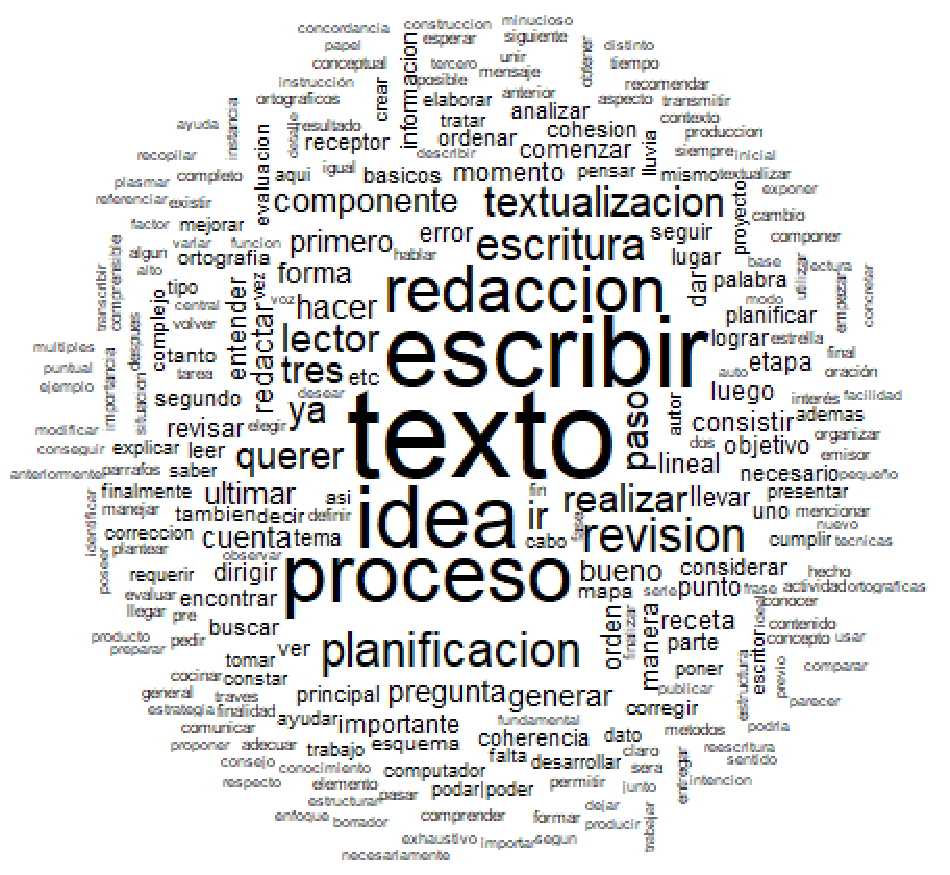
\includegraphics[width=0.5\textwidth]{figure01.pdf}
 \caption{Frecuencia de aparición del léxico especializado en el corpus.}
 \label{fig01}
 \source{elaboración própria.}
\end{figure}


\subsection{Léxico académico y resultados globales de la evaluación escrita}\label{sec-lex-aca-res}
En este apartado, la \Cref{fig02} da cuenta de la relación existente entre la
evaluación de los textos, considerando tanto el contenido como los aspectos
vinculados con la redacción, y la presencia de léxico académico. De los datos
obtenidos, se destaca que las líneas para cada elemento son, en general,
bastante similares, pero con un promedio más bajo en el componente léxico. En
este sentido, destacan los resultados del estudiante 15,quien obtuvo el puntaje
total para ambas dimensiones, así como los puntajes del estudiante 32, que
obtuvo sobre el 80\% de logro tanto para la producción textual como para el
léxico académico. A pesar de lo anterior, no podemos establecer una
relación directa entre léxico académico y calidad textual, pues una
generalización de ese tipo dejaría de lado las diferencias de puntaje que
evidencian los estudiantes 3, 7, 11, 19, 25 y 35, quienes presentan una
distancia considerable entre el puntaje global de sus escritos y la presencia de
léxico académico.

\begin{figure}[htbp]
 \centering
 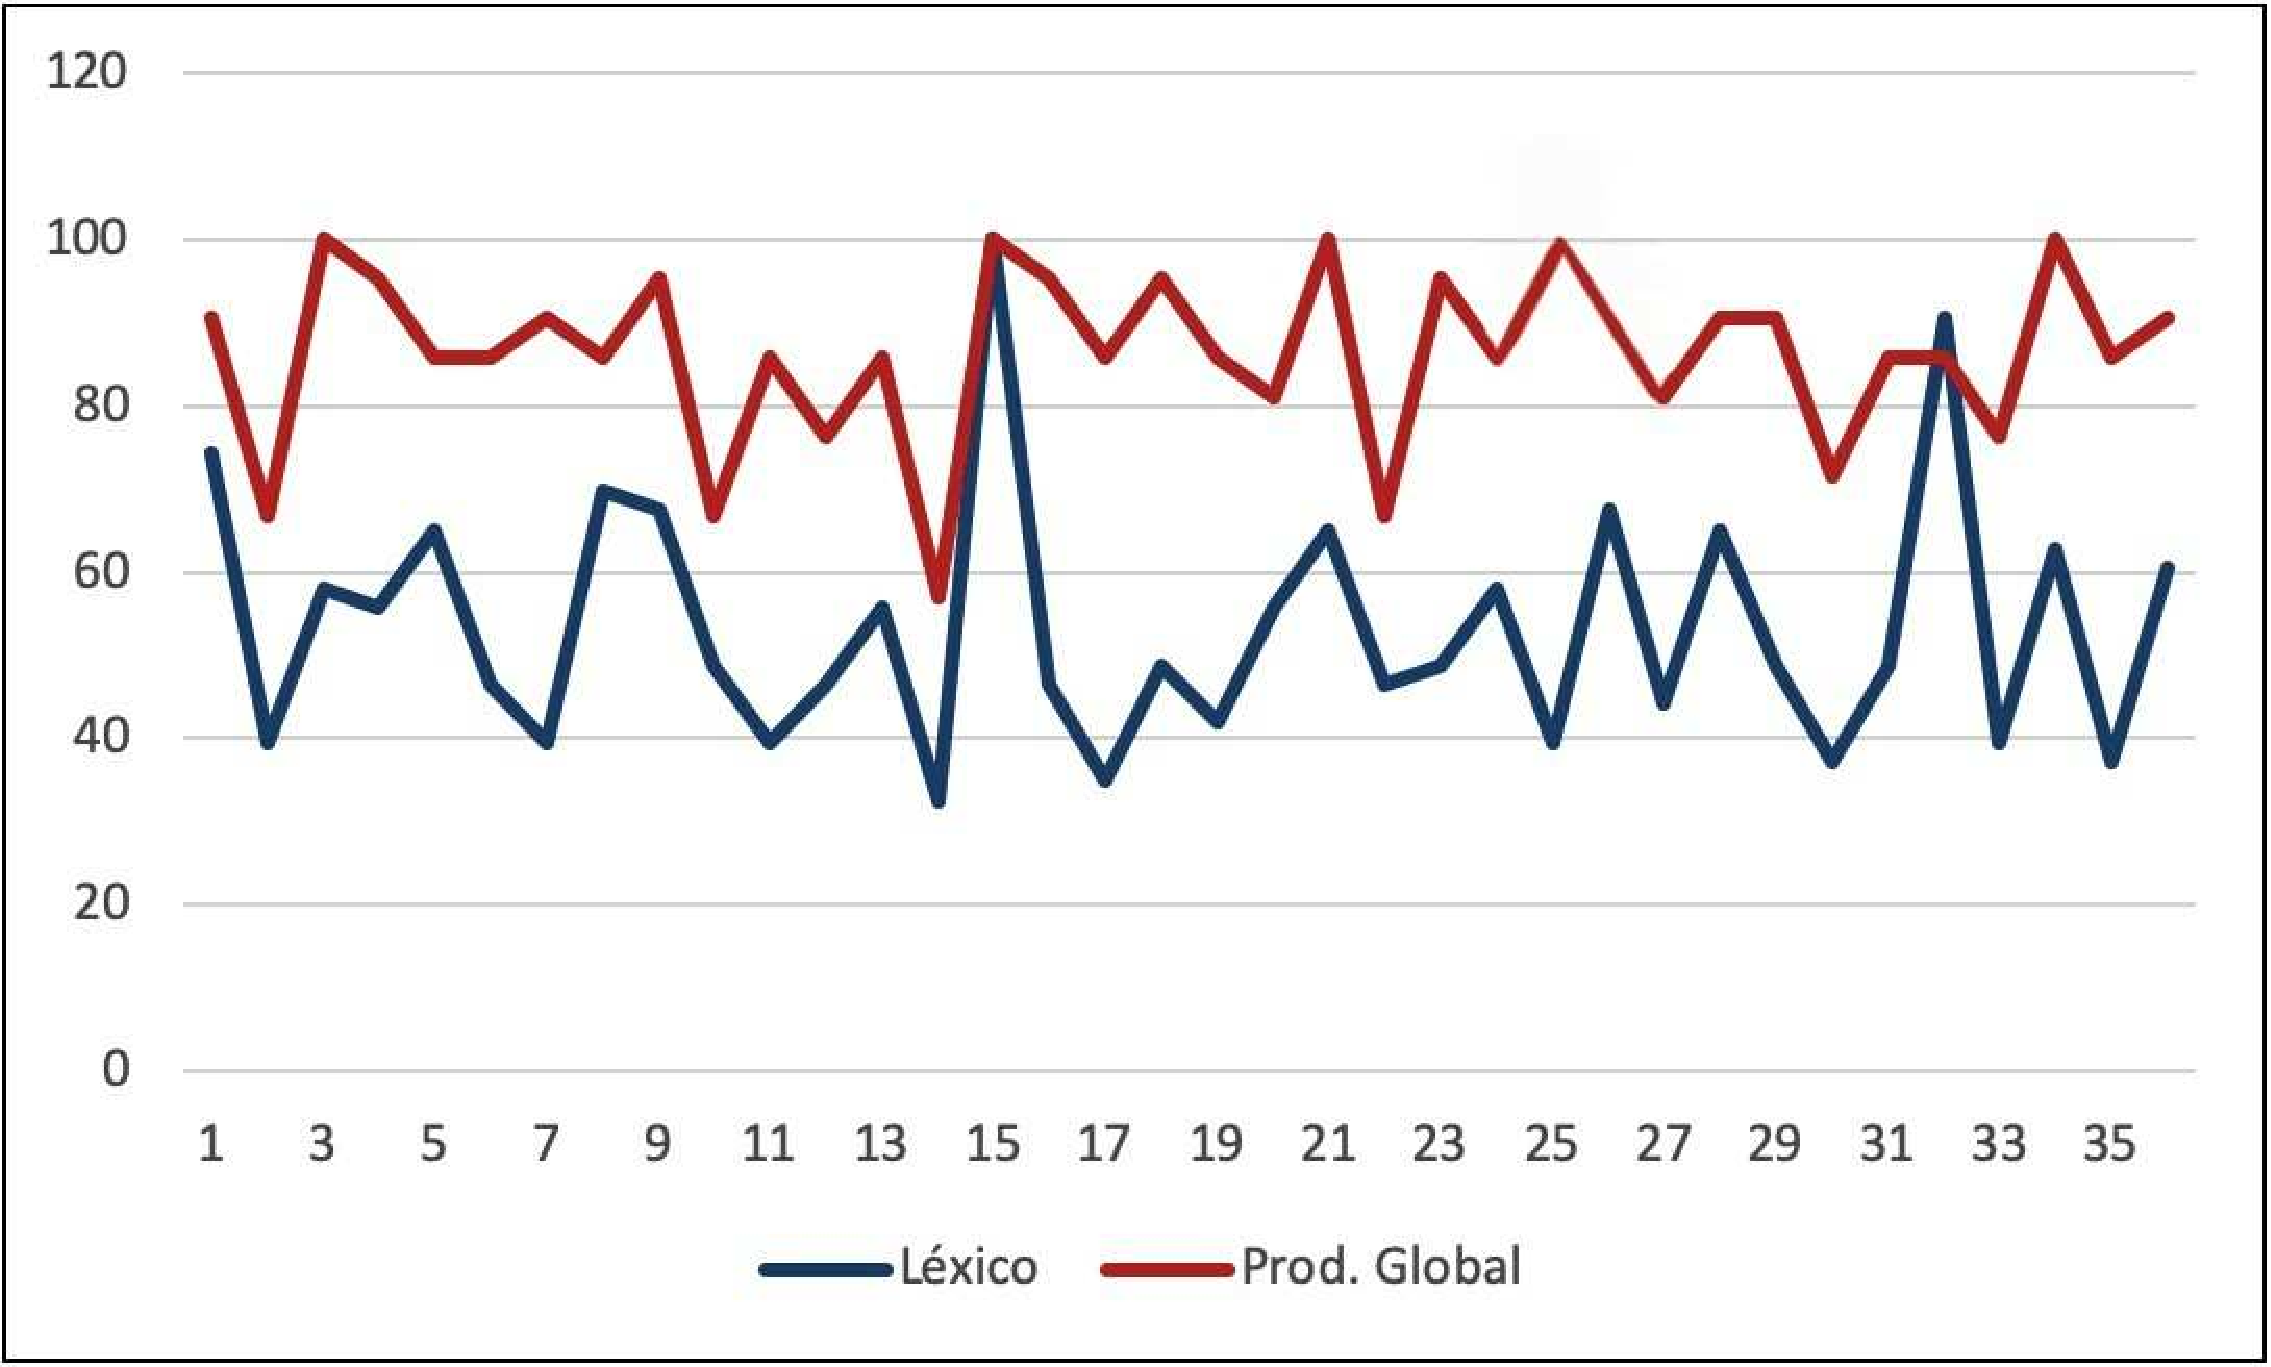
\includegraphics[width=0.6\textwidth]{figure02.pdf}
 \caption{Relación entre léxico académico y calidad global de los textos.}
 \label{fig02}
 \source{elaboración propria.}
\end{figure}


\subsection{Léxico académico y contenido de los textos}\label{sec-contenido}
En el caso del vínculo entre léxico académico y contenido de los textos,
se evidencia una relación bastante más estrecha (\Cref{fig03}). Se observa no solo
que las líneas son más cercanas, sino también que los casos en los que existe
puntaje distante son mucho menores: estudiantes 11, 17, 18, 19, 25 y 35.

Un caso particularmente llamativo es el del estudiante 25, quien obtuvo un
100\%de logro en el contenido, pero tan solo un 40\% en el componente léxico.
Esta diferencia podría explicarse debido a que el método que utilizamos para
evaluar esta última dimensión solo toma en cuenta la presencia de palabras
exactas, por tanto, la sinonimia, correferencia y otros mecanismos de cohesión
no fueron considerados. Esta idea se refuerza cuando volvemos a la \Cref{fig02},
pues se evidencia que el estudiante en cuestión presenta un alto nivel en la
calidad global de su escrito, lo que podría redundar en un variado uso de
mecanismos de cohesión.

\begin{figure}[htbp]
 \centering
 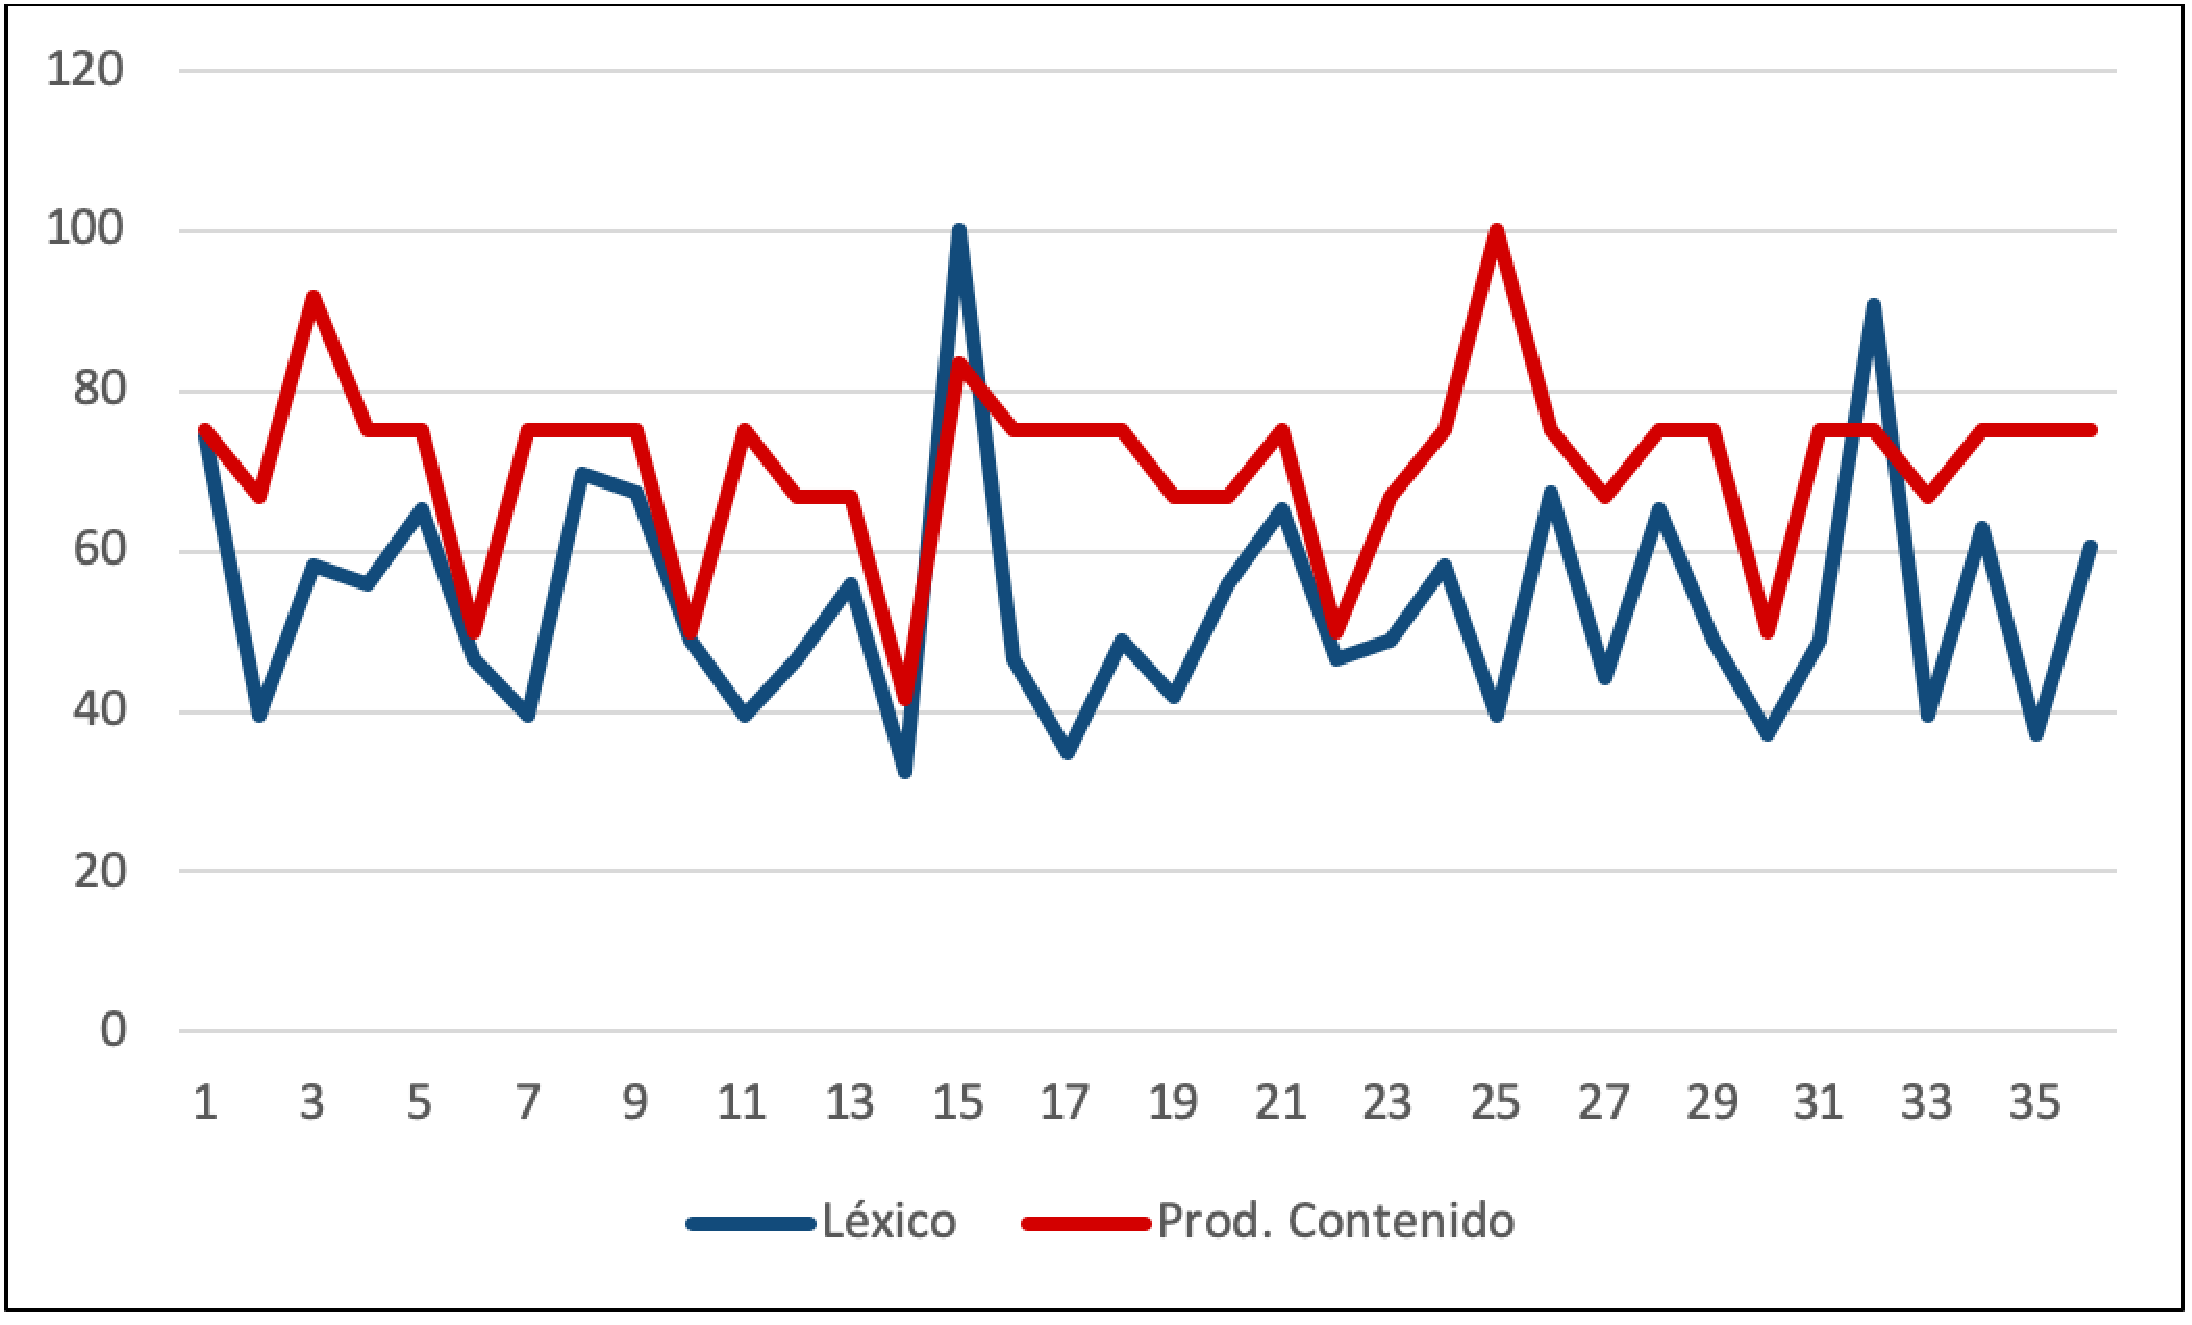
\includegraphics[width=0.6\textwidth]{figure03.pdf}
 \caption{Relación entre léxico académico y contenido de los textos.}
 \label{fig03}
 \source{elaboración propria.}
\end{figure}


\subsection{Léxico académico y calidad textual}\label{sec-calidad}
Respecto de esta relación, nos parece interesante destacar que no se
evidencia una tendencia clara (\Cref{fig04}): por una parte, hay estudiantes que
demuestran resultados muy cercanos entre léxico académico y la calidad textual
de su escrito (1, 2, 5, 8, 15, 32);mientras que, por otra, algunos dan cuenta
de resultados bastante alejados (4, 5, 6, 11,17, 18, 19, 25, 30, 35).

\begin{figure}[htbp]
 \centering
 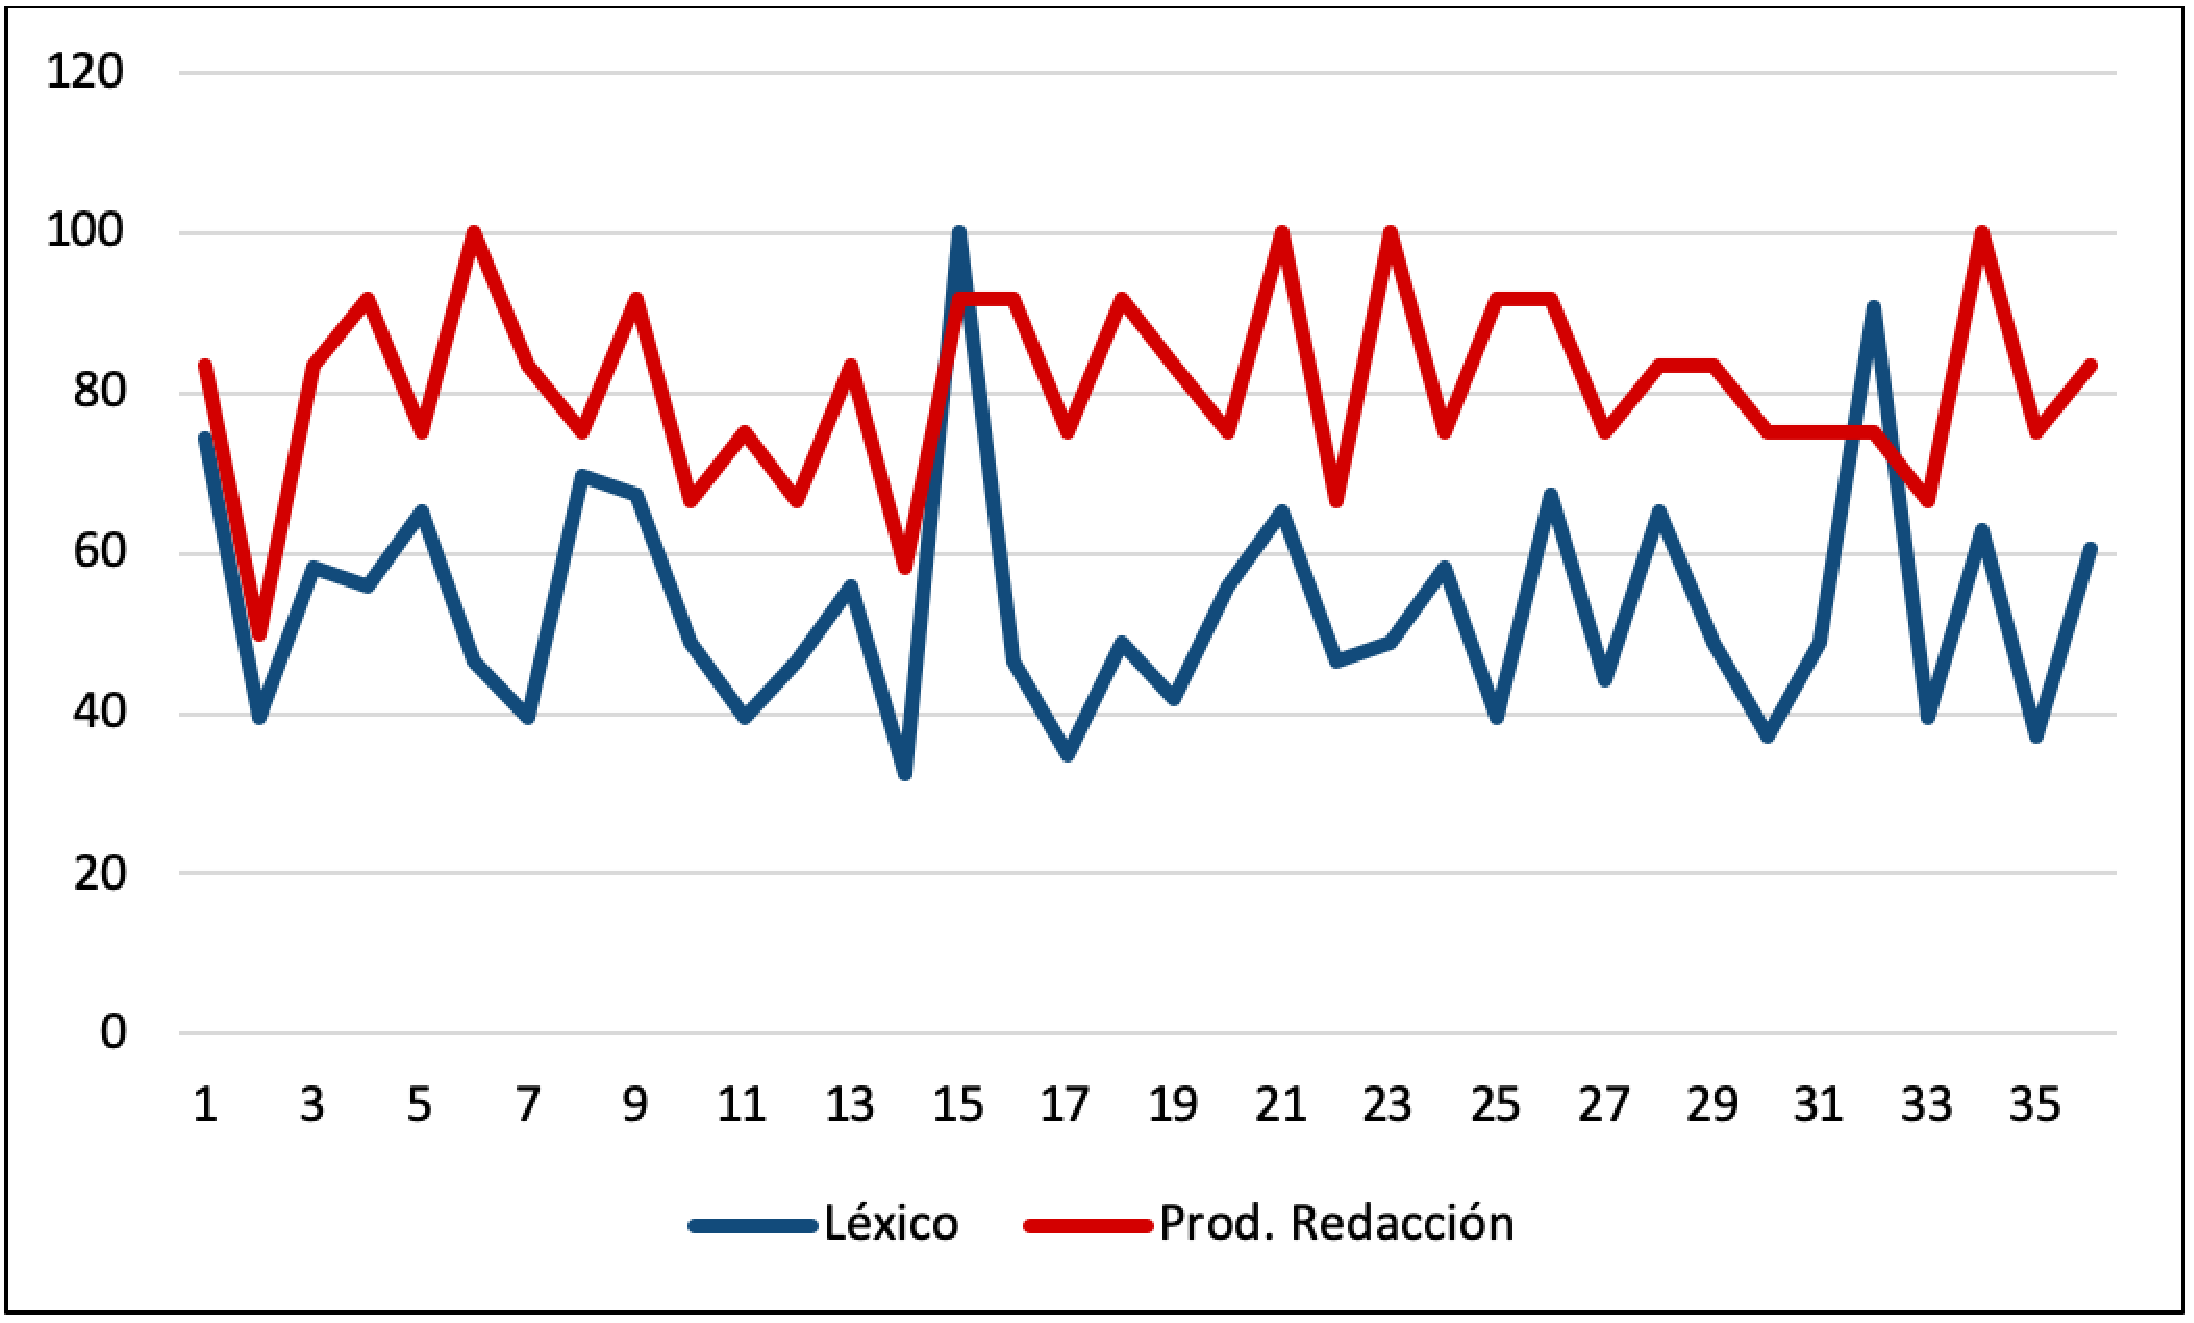
\includegraphics[width=0.6\textwidth]{figure04.pdf}
 \caption{Relación entre léxico académico y calidad textual.}
 \label{fig04}
 \source{elaboración propria.}
\end{figure}


\section{Discusión}\label{sec-discusion}
La relación entre competencia léxica y escritura ha sido profusamente estudiada
en el ámbito de la lengua inglesa y de la enseñanza de una segunda lengua. Si
nos enfocamos en el plano de la escritura académica, trabajos como el de \textcite{PrezCaado2010,Yoon2018,Pan2019}, 
entre muchos otros, se han centrado en
distintos aspectos de la escritura académica y su relación con la competencia
léxica: aprendizaje virtual y desarrollo del léxico, desarrollo de la escritura
en L2 y presencia de \textit{lexical bundles} en textos académicos, respectivamente. En
nuestra lengua, estudios sobre competencia léxica en la educación superior –
como el de \textcite{RiffoOcares2014,munoz2015,GonzaloZapico2016,Zapico2017,vega2018,Trigo2019},
entre otros muchos –, dan cuenta de la influencia que los estudios sobre
disponibilidad léxica han tenido en el ámbito de la educación a través de
la utilización de metodologías cuantitativas que miden el léxico mediante
evaluaciones específicas.

En contraste, más escasos resultan los trabajos que ponen el foco en el
léxico desde una perspectiva integrada \cite[p. e.]{madrigal2016,gracia2019},
perspectiva que adopta también la presente investigación. Un aporte
interesante al respecto es el que realizan \textcite{aravena}, quienes se
enfrentan al estudio del léxico en su contexto comunicativo y, sobre esa base,
relevan la importancia que tiene esta competencia en el desarrollo de
habilidades comunicativas complejas, como la adquisición de una segunda lengua
o el desempeño en lectura y escritura, desempeño que incide directamente en el
rendimiento académico (p. 199). 

En cuanto a la relación entre dominio léxico y calidad textual, nos
parece interesante destacar que un texto con mayor riqueza léxica o, en el caso
del corpus analizado, con mayor presencia de léxico académico, “no
necesariamente [...] va a estar bien realizado, pues habría que tomar en cuenta,
además, la cohesión y coherencia, el uso del componente notacional, así como la
puesta en práctica de requisitos gramaticales normativos” \cite[p. 145]{madrigal2016}.
Lo anterior se refuerza al observar los hallazgos de
\textcite{LilloFuentes2020}, quienes realizan una investigación en la
que valoran la calidad de la escritura de trabajos finales de grado de una
carrera del área de la ingeniería y la relacionan con rasgos
lingüístico-discursivos. En lo concerniente al vínculo calidad-riqueza léxica,
los autores señalan que “existe una correlación negativa entre el número de
palabras del escrito y la calidad de la escritura, por lo que las
introducciones que poseen mayor extensión, tienden a catalogarse de baja
calidad” \cite[p. 11]{LilloFuentes2020}.

Tomando en cuenta lo anterior, tanto nuestra investigación como la de
estos autores parecen evidenciar que unidades léxicas con contenido no nocional,
como conectores, pronombres, etc., tienen una mayor incidencia en aspectos como
la cohesión,lo que, a su vez, repercute directamente en la calidad de un texto.
En la misma línea, una investigación desarrollada hace varias décadas en un
contexto enseñanza de inglés como L2 señala entre sus hallazgos que los ensayos
redactados por estudiantes cuyas habilidades de escritura se ubican en niveles
avanzados suelen tener un alto número de conectores y pronombres \cite{Reid1992}.
Esto podría explicar perfectamente los resultados de estudiantes que, pese a
evidenciar un alto nivel de desempeño en su escritura, dan cuenta de una baja
presencia en cuanto a léxico académico (e.g., estudiantes 4, 5, 6, 11,17, 18,
19, 25, 30, 35 en la \Cref{fig04}). Sin duda, esta reflexión invita a indagar en
la relación entre calidad textual y léxico no nocional en textos producidos por
estudiantes universitarios de nuevo ingreso.

Sobre esta base, más que confrontar los resultados del presente trabajo con
los que obtuvieron \textcite{RiffoOcares2014,Giammatteo2003,GonzaloZapico2016,Wood2019}
– entre otros en los que se
correlaciona positivamente la competencia léxica con diferentes aspectos de la
competencia comunicativa (productiva y receptiva) –, nos inclinamos por destacar
que existe mayor incidencia del léxico académico en uno de los aspectos de la
competencia comunicativa escrita: el contenido textual.

Si bien estos resultados no son generalizables dadas las características
del estudio, es posible encontrar en la literatura una profusa cantidad de
trabajos que relacionan el léxico especializado con el dominio disciplinar,
sobre todo si consideramos en este ámbito lo mucho que se ha escrito sobre
alfabetización académica \cite{cantis2013,Baker2019,Kse2019}.
La relación que es posible establecer entre léxico académico, contenido
textual e incorporación de los aprendientes en una comunidad discursiva bien la
identifica \textcite[p. 55]{acevedo2006}, quien realiza un estudio en el que analiza
patrones léxicos en 163 trabajos de jóvenes universitarios y concluye que la
utilización de terminología de cada especialidad da cuenta del “nivel
de especialización alcanzado por los autores de los informes”.

En síntesis, los resultados de esta acotada experiencia nos entregan
información valiosa, desde el punto de vista pedagógico, sobre la importancia
que el léxico académico evidenció en el nivel de logro en el plano del
contenido de los textos, lo que, a su vez,incidió positivamente en la
evaluación global de los trabajos. Sin embargo, esta relación no llega a ser
determinante, pues hay antecedentes en la literatura especializada que relevan
una alta presencia de léxico no nocional en textos de alto nivel, lo que
podría explicar la distancia entre la calidad textual y el léxico disciplinar en
el corpus con el que hemos trabajado.



\section{Conclusiones}\label{sec-conclusiones}
Las analíticas de aprendizaje que hemos generado a través del software
Iramuteq – tanto la \Cref{fig01}, que da cuenta de la frecuencia del léxico
académico, como las restantes, que evidencian el desempeño en una tarea de
escritura –, nos permiten establecer que los textos analizados presentan una
relación estrecha entre léxico académico y calidad del contenido de los textos,
No obstante, a nivel de calidad textual(vale decir, considerando ortografía,
extensión, coherencia y cohesión y organización y estructura), la influencia del
léxico académico resulta menos determinante. Esto nos invita a reflexionar en
torno al nivel de incidencia que el léxico no nocional (vale decir,conectores,
pronombres, preposiciones, etc.) tiene en la calidad de los textos, por lo
que se abre una interesante línea para futuros trabajos.

Finalmente, cabe precisar que, si bien el diseño de la investigación no nos
permite generalizar los resultados, estos ofrecen datos interesantes en lo
relativo a la importancia que el desarrollo de la competencia léxica académica
posee en los procesos de alfabetización académica de los estudiantes
universitarios, sobre todo, considerando los indicios que entrega esta
competencia en relación con el dominio disciplinar.


\printbibliography\label{sec-bib}
% if the text is not in Portuguese, it might be necessary to use the code below instead to print the correct ABNT abbreviations [s.n.], [s.l.] 
%\begin{portuguese}
%\printbibliography[title={Bibliography}]
%\end{portuguese}

\end{document}
